\section{Preprocessing dei dati}
\label{sec:pre-proc}

I dati analizzati, forniti dall'ufficio XXX\scolli{specificare il nome dell'ufficio}, 
erano organizzati in formato Excel con una struttura tabellare complessa, contenente 
numerosi campi. Per garantire un'analisi efficace e accurata, si è resa necessaria una 
fase di preprocessing, finalizzata a correggere eventuali incoerenze, migliorare la 
qualità complessiva del dataset e suddividerlo in sottoinsiemi più gestibili.

Il dataset fornito includeva informazioni relative ai docenti, ai ricercatori e alle 
coperture degli insegnamenti nei diversi corsi di laurea. Dopo un'attenta analisi 
preliminare, sono stati selezionati esclusivamente i campi considerati rilevanti per 
l'analisi. Nel file contenente i dati di docenti e ricercatori, sono state prese in 
considerazione solo le informazioni riguardanti la matricola, la fascia contrattuale 
e l'SSD. Per quanto riguarda il file sulle coperture, sono stati mantenuti i campi 
relativi alla matricola del docente, al codice del tipo di corso, al codice del 
di laurea e all'SSD.

Questa selezione dei dati è stata essenziale per ridurre la complessità e concentrarsi 
sugli elementi chiave necessari per costruire il modello ASP e verificare il rispetto 
dei vincoli ministeriali. Tutto questo è stato realizzato utilizzando diversi script in 
Python, supportati dai moduli \texttt{pandas}\footnote{\url{https://pandas.pydata.org/}} 
e \texttt{openpyxl}\footnote{\url{https://openpyxl.readthedocs.io/en/stable/}}, 
essenziali per la manipolazione e la gestione dei dataset.

La maggior parte delle operazioni di preprocessing ha riguardato il file contenente 
le coperture degli insegnamenti, articolandosi in diverse attività principali. 
In primo luogo, abbiamo gestito le righe contenenti una o più colonne vuote, 
eliminando quelle completamente prive di informazioni, in quanto non rilevanti 
per l'analisi. Le righe in cui mancavano i dati relativi al docente (i.e., matricola, 
nome e cognome) sono state invece isolate in un file separato. Questa scelta è stata 
necessaria per identificare e analizzare in modo specifico gli insegnamenti non 
ancora assegnati ad alcun docente.

Un ulteriore passo fondamentale ha riguardato la scomposizione del dataset originale, 
suddividendolo in sottoinsiemi più piccoli e gestibili. Questa operazione ha permesso 
di affrontare con maggiore precisione i singoli aspetti del problema, semplificando il 
successivo trattamento dei dati. Infine, sono stati identificati e gestiti in modo 
univoco e automatizzato i casi particolari, consentendo di creare un dataset uniforme 
e privo di anomalie, adatto all'analisi e all'implementazione del modello ASP.

Per migliorare ulteriormente la gestibilità dei dati, abbiamo proceduto con la creazione 
di sottoinsiemi minimali e distinti. Il primo passo è consistito nella separazione delle 
righe relative agli insegnamenti tenuti da docenti o ricercatori da quelle tenute dai 
docenti a contratto.

Questa suddivisione è stata effettuata utilizzando il file dei docenti fornito, 
sfruttando la colonna contenente la matricola come criterio discriminante. In particolare, 
le righe associate ai docenti a contratto sono state estratte e archiviate in un file separato, 
al fine di garantire un maggiore ordine e facilitare eventuali ispezioni manuali. 
Parallelamente, le righe relative ai docenti a tempo indeterminato e determinato sono 
state salvate anch'esse in un altro file, per gli stessi identici motivi.

Una volta completata la suddivisione, è stata apportata una modifica ai valori nella colonna 
relativa al codice del tipo di corso di laurea. In particolare, tutte le occorrenze del 
valore \texttt{L} sono state sostituite con \texttt{LT}, così da esplicitare i corsi di 
laurea triennale e migliorare la chiarezza dei dati. Successivamente, abbiamo proceduto con 
l'identificazione dei casi particolari utilizzando un controllo incrociato tra due colonne 
specifiche. Questo processo ha permesso di individuare e gestire in modo univoco i corsi 
di laurea che presentano requisiti particolari, come illustrato nella 
Figura~\ref{fig:casi_particolari}.
Per implementare questa logica, abbiamo adattato il processo di modifica dei dati al corso 
specifico da verificare. Ad esempio, per la Laurea Triennale in Servizio Sociale, abbiamo 
sostituito il codice del tipo di corso precedentemente identificato come \texttt{LT} con 
\texttt{LTSS}.

\begin{figure}[h]
    \centering
    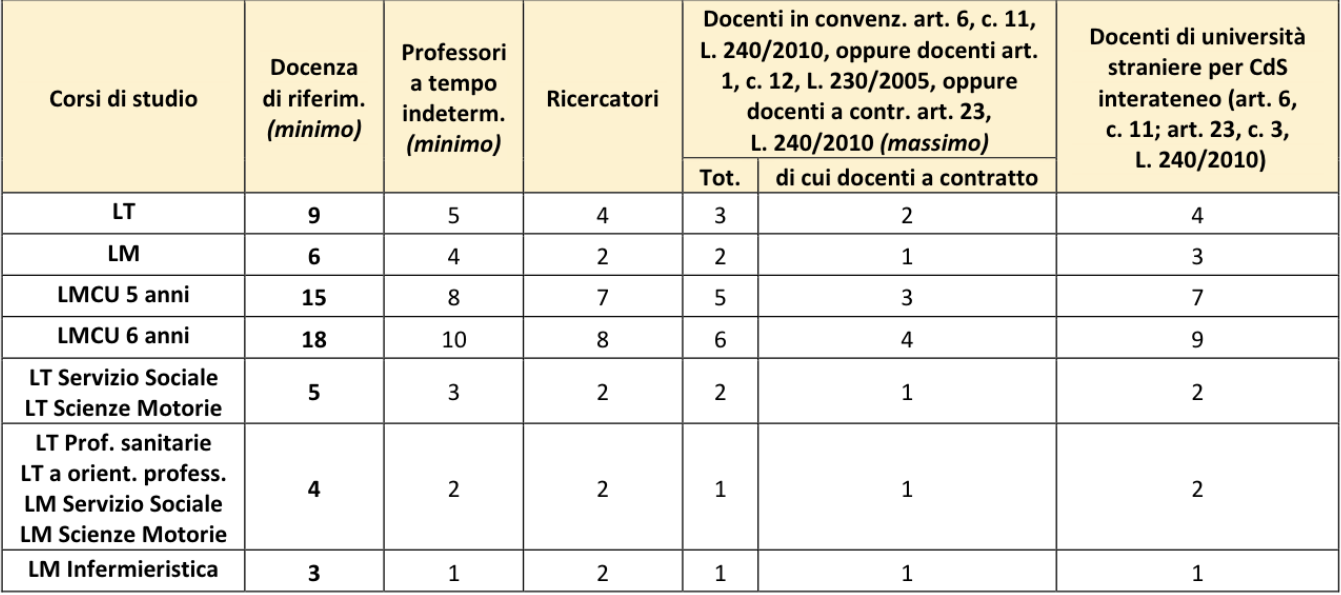
\includegraphics[width=0.8\textwidth]{./images/tabellaministeriale.png}
    \caption{Casi particolari}
    \label{fig:casi_particolari}
\end{figure}


\mmerenda{aggiungere la roba nuova discussa nella call con l'ufficio del 06/12/2024}